\chapter{Statusseminar}
\section{Baggrund}
Projektet formål er at udvikle en algoritme til kategorisering af lægemiddelskift. På nuværende tidspunkt vurderes kompleksiteten ved lægemiddelskift af ATC-eksperter og er derfor meget personafhængig. En algoritme kan derfor anvendes som et hjælpemiddel til ATC-eksperterne i forhold til at kategorisere i hvilke tilfælde de skal være særligt opmærksomme på et lægemiddelskift. Med særligt opmærksomme menes der hvilke foretag eller informationer, som skal videregives til klinikken ved et lægemiddelskift med henblik på at forebygge eventuelle medicineringsfejl. 

\section{Problemanalyse}
Den stigende andel af ældre, forekomsten og varigheden af kroniske sygdomme samt udviklingen i sundhedsforventninger og teknologier er skyld i stigende sundhedsudgifter i flere europæiske lande~\citep{Ess2003}. Siden år 2007 til 2015 har udgifterne til sygehusmedicin steget 7,8~\% i gennemsnit om året~\citep{Sundhed2016}.

For at begrænse udgifterne har Amgros, Regionernes lægemiddelorganisation, siden år 2007 sendt lægemidler i udbud årligt med henblik på at indkøbe lægemidler af høj kvalitet til bedst mulige pris til de offentlige danske hospitaler~\citep{Sygehusapoteket2017}. Udbud forekommer på lægemidler, hvor der findes mere én leverandør, hvormed lægemidler bringes i konkurrence, hvilket kan give anledning til et kontraktskift~\citep{Amgros2015}. 

Kontraktskift medfører substitution af lægemidler, hvilket betyder udskiftning af et lægemiddel til et andet~\citep{DanskSelskabforPatientsikkerhed2009}. 
Generisk substitution, hvor to lægemidler indeholder samme virksomme stof, er den hyppigste form for substitution. Denne form kræver ikke recept og kan varetages af en sygeplejerske.~\citep{DanskSelskabforPatientsikkerhed2009} 

Der er patientsikkerhedsmæssige konsekvenser forbundet med generisk substitution, herunder fejlmedicinering~\citep{Hakonsen2010}. 
Den hyppigste fejl ved generisk substitution skyldes i 82,1~\% af tilfældene forkert lægemiddel~\citep{Hakonsen2010}. De typiske anledninger til forket lægemiddel er forveksling af emballager eller navne, hvilket i nogle tilfælde har medført forlænget indlæggelse, forværret sygdom og dødsfald~\citep{DanskSelskabforPatientsikkerhed2009}.

Informationssystemer har påvist at være anvendeligt i forebyggelse af medicineringsfejl~\citep{Agrawal2009}. Dette indebærer f.eks. computerbaseret lægeordreindgang, automatisk dispenseringsskabe, bar-kodet medicin administration samt elektronisk afstemning af medicin.~\citep{Agrawal2009} Klinisk beslutningsstøtte, som f.eks. i form af advarsler, har påvist at forbygge forveksling af navn og styrke og ligeledes at reducere antallet af medicineringsfejl~\citep{Campmans2018}.
\textcolor{red}{Lina: Synes du der mangler noget i forhold til at forstå problemet? Dette skal være en kort opsummering af baggrundsmaterialet}

\subsection{Problemformulering}
\centering \textit{Hvilket potentiale har en algoritme til kategorisering af lægemiddelskift?}

\section{Data}
Data er indsamlet af Amgros og Sygehusapoteket Region Nordjylland og består af flere excelark, hvor data skal udtrækkes fra og indgå i algoritmen. Forskellige faktorer vægtes alt efter hvor kompleks håndteringen af lægemiddelskiftet er. Denne vægten er foretaget i samarbejde med en ekspert på området. Følgende faktorer skal inkorporeres i algoritmen: 
\begin{enumerate}
\item \label{1} \textbf{Navneændring}: Dette kan give anledning til forvekslinger, hvorved den forkerte medicin kan dispenseres.
\begin{enumerate}
\item \textbf{Sound-a-like}: Ved navneændring ønskes der yderligere at beregne Levenshtein distancen for at kunne sammenligne om det nye navn er fuldstændig ændret og/eller om der allerede eksisterer et lignende navn (Den sidste nævnte skal kombineres med dispenseringsform, da det er i disse tilfælde fejl kan opstå).
\end{enumerate} \vspace{2mm}
\item  \textbf{Pakningstrørrelse, styrke, dispenseringsform}: Samme begrundelse som ved punkt \ref{1}. Disse vægtes dog forskelligt, da pakningsstørrelse primært skyldes pladsmangel i klinikkerne, hvor styrke og dispenseringsform kan give anledning til komplikationer for patienten, hvis disse dispenseres forkert \vspace{2mm}
\item \textbf{Analogskift:} Analog substitution er lægemidler med beslægtet kemi og ensartet klinisk virkning. Disse adskiller sig fra generiske som har nøjagtig samme indholdsstof, hvorfor der skal være særligt opmærksomhed rette mod disse. \vspace{2mm}
\item \textbf{Risikolægemidler}: Disse lægemidler kan være problematiske, hvis de ender i restordre, altså at det er nødvendigt at finde et erstatningslægemiddel \textcolor{red}{Lina: Jeg ved ikke helt om dette skal med, tænker måske det forvirre dem mere, da det omhandler restordre lige pludselig eller kan jeg omformulere mig her? Måske skrive udsolgt/leveringssvigt i stedet for restordre? Hvad tænker du?}\vspace{2mm}
\item \textbf{Komplekse ATC-koder}: Der er nogle ATC-koder som er mere komplekse end andre. Dette er f.eks. på kræft og væske området, da disse områder .... . \textcolor{red}{Lina: Har lidt svært ved at finde en begrundelse - kræftområdet er vel primært fordi det er dyrt? Og væske er fordi det anvendes på mange afdelinger eller?... Kan ikke lige huske den..} ATC-koderne er indsamlet via dokumenterede problemstillinger ved disse.
 \vspace{2mm}
\item \textbf{Medicinråd}: En lille del af lægemidler omhandler medicinrådets behandlingsvejledninger. Disse lægemidler skal implementeres i klinikken og omfatter enkelte hospitalsafdelinger. Det ønskes at disse implementeres hurtigt, da det er muligt at opnå store besparelser. \vspace{2mm}
\item \textbf{Pris}: Pris er vigtigt i forhold til at opnå besparelser. Det skal ligeledes vægtes om det kan betale sig at skifte et lægemiddel med mindre besparelse, da udskiftningen kan få store betydninger for klinikken i forhold til arbejdsgangen og i værste tilfælde medføre patientsikkerhedsmæssige konsekvenser. \textcolor{blue}{Det er endnu ikke besluttet, hvordan denne faktor skal inkorporeres i algoritmen. Det er svært at måle besparelse.}\vspace{2mm}
\end{enumerate}

\section{Algoritme}
Algoritmen vil opbygges på baggrund af et regel-baseret system. %Regel-baseret systemer er nyttige og effektive på områder som kræver symbolsk behandling af viden~\citep{Ligeza2006}.
Udviklingen af regel-baseret system er baseret på fem trin~\citep{Ligeza2006}, som er fremgår af Figur \ref{fig:metode}.  

\begin{figure}[H]\centering	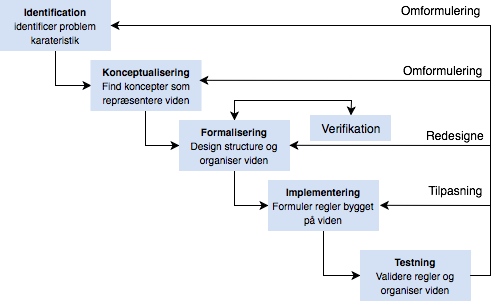
\includegraphics[width=0.7\textwidth]{Statusseminar/metode.png} 
	\caption{De fem trin for udviklingen af regel-baseret system.~\citep{Ligeza2006}}
	\label{fig:metode}  
\end{figure}
\vspace{-0.5cm}
Første trin omhandler identificering af problemer som systemet skal løse, herunder data som systemet skal arbejde på og tilgængelige ressourcer~\citep{Ligeza2006}. Det andet trin er omhandler identificering af nøglekoncepter samt relationer mellem disse som f.eks. typer af data, informationsstrøm og underliggende stukturer. Tredje trin involverer forståelse, beskrivelse og formalisering af problemet og hvordan løsninger findes. Denne proces bør omfatte verificering af systemet. Det fjerde trin har til formål at implementere den formaliseret viden i et program. Det sidste trin omfatter test ved validering af regler og implementeringen.~\citep{Ligeza2006}
 
\section{Samarbejde}
Projektet er et ekstern samarbejde med Sygehusapoteket Region Nordjylland. I projektet samarbejdes med en MedIS-studerende (Translationel Medicin) som udarbejder interview og fokusgruppeinterview i forhold til at vurdere, hvornår et lægemiddelskift er kompleks. Disse interview skal danne grundlag for vægtningen af parameterne i algoritmen. 

Yderligere skrives et projekt omhandlende samme område af en projektleder i lægemiddelinformation. Dette projekt bygger også på interviews og fokusgrupper og skal ende ud i en udarbejdelse af metodehåndbøger for tiltag i klinikken i forbindelse med lægemiddelskift.\textcolor{red}{Tror du jeg siger for meget her i forhold til hvad jeg må omkring Emilies projekt?}

\section{Projektplan}
På nuværende tidspunkt i projektet arbejdes der på det tredje trin, jævnfør Figur \ref{1} med henblik på snart at indlede fjerde trin. Samtidig med udviklingen af algoritmen arbejdes der stadig på indsamling af viden på forskellige områder i forhold til problemanalysen samt metode.



